\chapter{Case study}

\section{Codon optimisation}
Recall the redundant mapping from codons to amino acid and the basic structure of a bacterial gene. In prokaryotes functionally related genes are often grouped in operons\footnote{a unit made up of linked genes which is thought to regulate other genes responsible for protein synthesis.}.
\subsection{Introduction to codon optimisation}
The amino acid code is redundant. Different organisms have different preferences for particular codons. The selection pressure is primarily on growth rate. It is the efficiency optimisation that the organism has done doing evolution. For example, match the codon usage of the gene construct and the host organism; Use the codons found in highly expressed genes.
\subsection{Which are the best codons to use}
A research by ATUM suggested that Genes differing only in synonymous codon usage expressed protein at levels ranging from undetectable to 30\% of cellular protein. It is not those codons most abundant in highly expressed \textit{E. coli} proteins that are the best codons to use, instead, it is the codons read by tRNAs that are \udl{most highly charged} under conditions of amino acid starvation.

\section{Recombinant Insulin}
\subsection{Introduction to Genetic Engineering}
Broadly, genertic engineering is the directed modification of an organism's genetic makeup.\\[.1in]
\udl{Recombinant protein expression} is the process of expressing non-native proteins in an organism. Treat the organism as molecular machine, into which specific DNA sequences are introduced. Introduce DNA with non-native genes, from which the cell will produce a non-native protein (aka \udl{heterologous} or \udl{recombinant protein})
\begin{enumerate}[itemsep=0mm]
    \item to produce a valuable protein product
    \item to create an organism with favourable properties.
\end{enumerate}
\subsection{Genetic Parts and Tools}
To enable recombinant protein expression, we need to create a functional gene.
\begin{figure}[h]
\centering
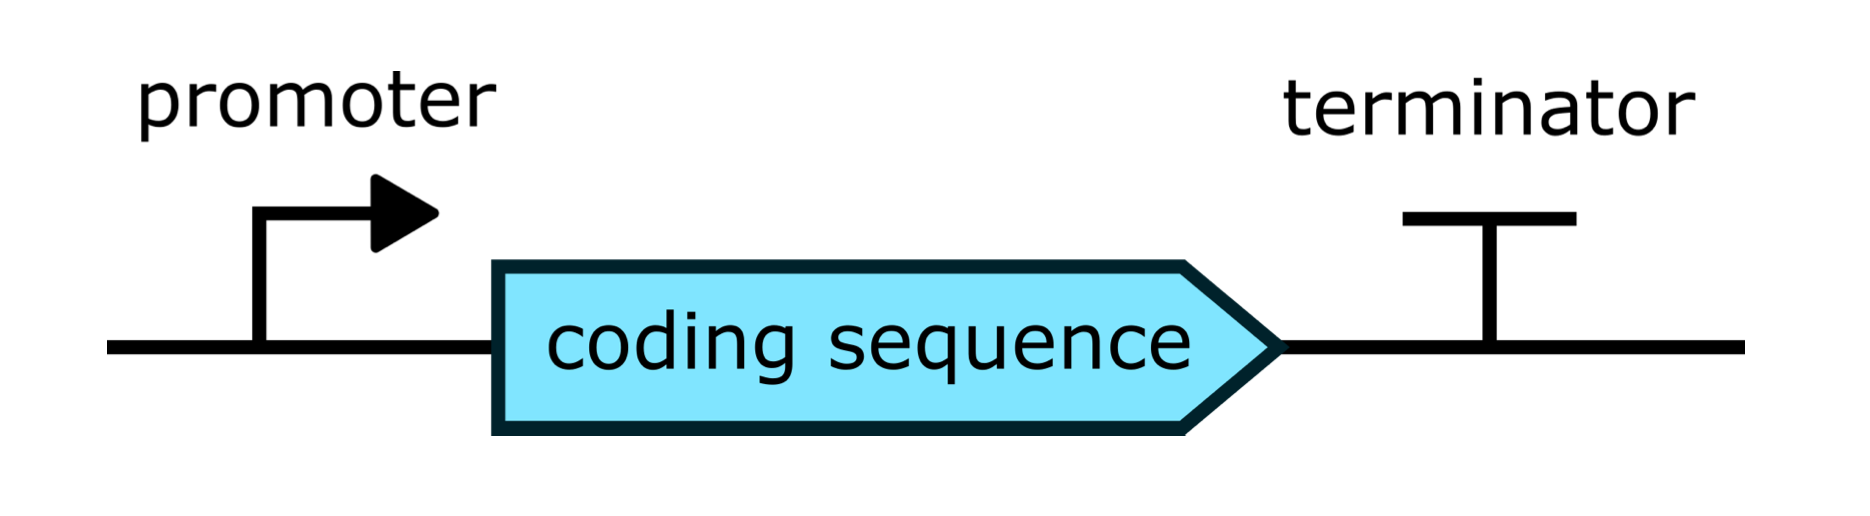
\includegraphics[width=0.8\textwidth]{images/5-1.png}\\[.2in]
\caption{Desirable gene structure}
\end{figure}
\FloatBarrier
\begin{itemize}
    \item Promoters - initiate transcription
    \begin{enumerate}
        \item Can be constitutive or regulated (P\textsubscript{Iac} is IPTG-inducible, P\textsubscript{BAD} is arabinose-inducible)
        \item Regulation enables control of protein expression
        \item Promoters have a range of 'strengths' that determine that levels of protein expressed
    \end{enumerate}
    \item Coding sequences (CDSs) - encode protein amino acid sequence
    \begin{enumerate}
        \item Also known as open reading frames (ORFs)
        \item Functional protein subdomains can be fused together
        \item Short tags direct proteins for specific cellular compartments in Eukaryotes
        \item Affinity tags facilitate the purification of recombinant proteins
    \end{enumerate}
    \item Terminators - stop transcription
\end{itemize}
\subsection{Coding Sequences (CDSs) -- Affinity Tags}
\begin{figure}[h]
\centering
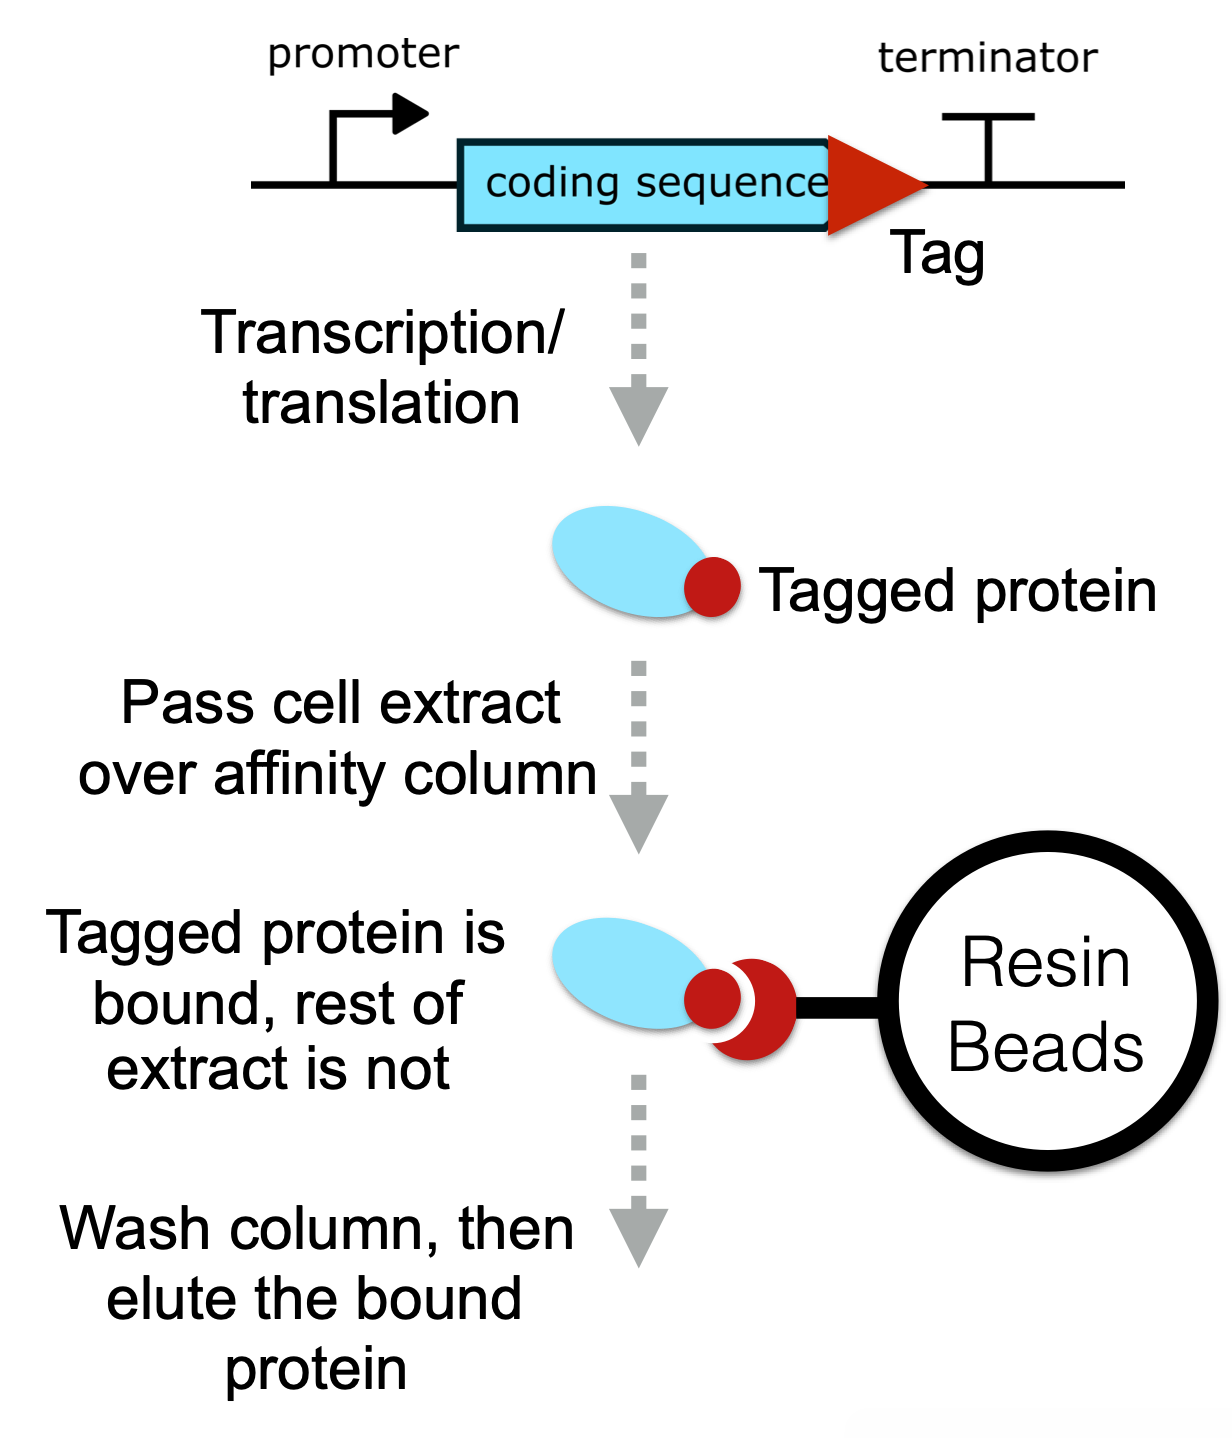
\includegraphics[width=0.5\textwidth]{images/5-2.png}\\[.2in]
\caption{Affinity Tags}
\end{figure}
\FloatBarrier
\begin{itemize}
    \item Affinity tags enable protein purification through interaction with solid phase. 
    \item Most often at N-terminus or C-terminus.
    \item e.g. 6x histidine tag binds Ni\textsuperscript{2+} ions immobilised\footnote{prevent (something or someone) from moving or operating as normal} on agarose resin. 
    \item 3xFLAG tag has enterokinase cleavage site allowing elution\footnote{remove (an adsorbed substance) by washing with a solvent} of the tag-free protein.
\end{itemize}
\subsection{Host Organisms}
Different host organisms or 'chassis' have different properties, choosing which to work with is important.\\[.1in]
% Table ---
\begin{table}[h]
\centering
\resizebox{0.9\textwidth}{!}{%
\begin{tabular}{@{}cll@{}}
\toprule
Organism & \multicolumn{1}{c}{Class} & \multicolumn{1}{c}{Properties} \\ \midrule
\textit{E. coli} & \begin{tabular}[c]{@{}l@{}}Gram-negative \\ bacterium\end{tabular} & \begin{tabular}[c]{@{}l@{}}Easy to grow, relatively simple cellular \\ physiology, numerous genetic tools\end{tabular} \\
\begin{tabular}[c]{@{}c@{}}\textit{S. cerevisiae}\\ (budding yeast)\end{tabular} & \begin{tabular}[c]{@{}l@{}}'simple' eukaryote\end{tabular} & \begin{tabular}[c]{@{}l@{}}Easy to grow, efficient protein \\ secretion, complex metabolism\end{tabular} \\
\begin{tabular}[c]{@{}c@{}}Mammalian cells\end{tabular} & \begin{tabular}[c]{@{}l@{}}complex eukaryote\end{tabular} & \begin{tabular}[c]{@{}l@{}}More difficult to grow, an produce \\ true human proteins\end{tabular} \\ \bottomrule
\end{tabular}%
}
\caption{Host organisms}
\label{tab:organisms}
\end{table}
\FloatBarrier
Eukaryotes are capable of various post-translational modifications (e.g. glycosylation, proteolytic processing) and use specific signals to direct proteins to be inserted into the membrane or secreted.
\subsection{Engineering recombinant insulin}
Diabetes mellitus is a common disorder that can be fatal if not treated. Many diabetics require daily injections of a peptide hormone insulin to regulate their blood glucose levels. Pig insulin used to be used to treat diabetics, but production methods were inconsistent and not cost-effective. Insulin was the \udl{first hormone} to be produced by recombinant DNA technology.
\subsection{Recombinant Insulin}
\bd{Design brief}
\begin{itemize}
    \item make recombinant insulin that can be produced in \udl{large volumes}, purified easily, \udl{functional in humans} and \udl{safe}.
    \item Using \textit{E.coli} as host
\end{itemize}
\bd{Issues}
\begin{itemize}
    \item preproprotein is processed into mature protein
    \item cleavage removes N-terminus (no methionine left)
    \item middle is proteolytically removed
    \item mature A and B polypeptides held together with disulfide bonds
\end{itemize}
Today, much of recombinant insulin is produced in the budding yeast. \textit{S.} \textit{cerevisiae}.

\section{Antibodies}
\subsection{Antibody immune response}
Antibodies have a number of effects on their targets. Antibodies form an important part of the \udl{adaptive immune response}.
\begin{enumerate}
    \item \bd{Neutralisation} \\ Antibodies prevent a virus or toxic protein from binding their target.
    \item \bd{Opsonisation} \\ A pathogen tagged by antibodies is consumed by a macrophage or neutrophil.
    \item \bd{Complement activation} \\ Antibodies attached to the surface of a pathigen cell activate the complement system.
\end{enumerate}
Antibodies (Abs) have natural properties that make them high useful:
\begin{itemize}
    \item Abs recognise antigens with exquisite specificity
    \item Abs are highly diverse with known structural properties
    \item Abs are robust molecules that are naturally long lived
    \item Abs are a normal part of the human immune system
    \item Around $10^{10}$ variants in humans
\end{itemize}
\subsection{Antibodies structure}
Antibodies is \udl{Y-shaped}. Proteins are produced by \udl{B cells}. They bind specific targets. They consist of \udl{two heavy and two light chains}. Different antibodies bind different antigens (Ag) based on \udl{variations in the antigen-biding site} (5). It has \udl{two identical Ag binding sites} increases Ab affinity\footnote{the degree to which a substance tends to combine with another.}.
\begin{figure}[h]
\centering
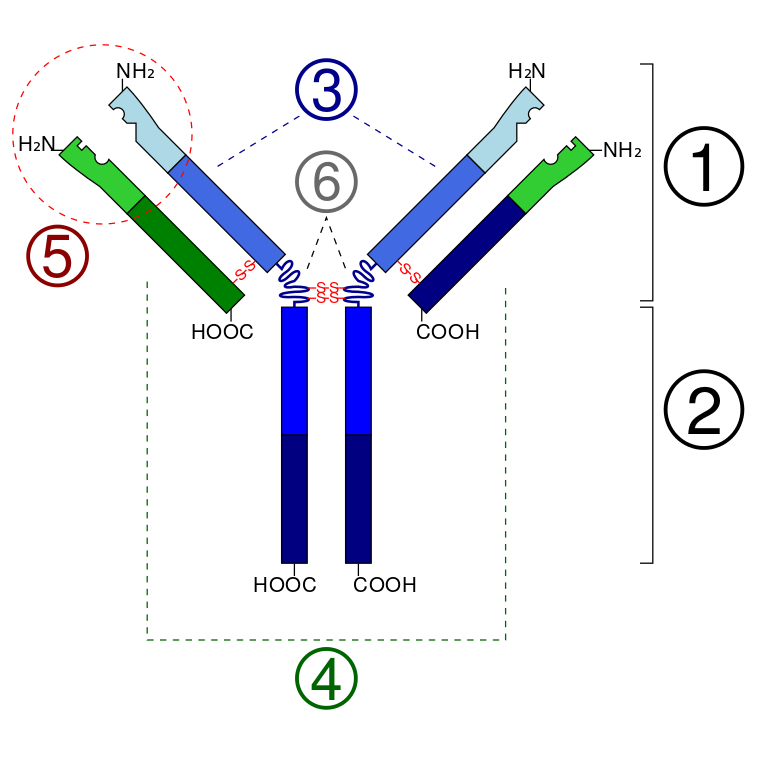
\includegraphics[width=0.6\textwidth]{images/Immunoglobulin_basic_unit.svg.png}\\[.1in]
\caption{Antibody structure}
\end{figure}
\FloatBarrier
\begin{enumerate}[noitemsep]
    \item Fragment antigen binding (Fab) region
    \item Fragment crystallisable (Fc) region
    \item Heavy chain (blue): 1 variable and 3 constant domains
    \item Light chain (green): 1 variable and 1 constant domain
    \item Antigen binding site
    \item Hinge region
\end{enumerate}
The heavy and light chains are composed of subdomains, each with a common beta-sheet rich immunogobulin (Ig) fold. The variable domain at the tip of each Fab arm has \udl{highly variable amino acid sequence}. This variation is what accounts for antigen specificity.
\subsection{Antibodies: Complementary Determining Regions}
The amino acid sequence of the complementarity determining regions (CDRs) aka \udl{hypervariable} regions dictate antigen specificity.
\subsection{Antibodies: gene to protein}
uring B cell maturation, \udl{\textit{somatic recombination}} leads to joining of gene segments at DNA level. Combinatorial diversity results in many possible amino acid sequences \udl{at the CDRs}. Heavy chain: 44x V, 27x D, 6x J segments each with different sequence. Light chain: many V, J segments (no D) -- Totally about \udl{$3\times10^{11}$ possibilities}. Affinity maturation (directed mutation) creates further diversity.
\subsection{Monoclonal Antibodies: Therapeutic uses}
\bd{Scale: Producing Monoclonal Antibodies (mAbs)}
\begin{enumerate}[itemsep=0mm]
    \item Challenge mouse with antigen.
    \item Purify Iymphocytes (B cells, motal, HGPRT+) from spleen.
    \item Fuse with myeloma cells (immortal, HGPRT-).
    \item Select for \udl{hybridoma clones} (fused cells, HGPRT+, immortal).
    \item Screen for antibody production against target antigen.
    \item Positive clones secrete \udl{monoclonal antibodies} into the culture medium and can be grown indefinitely.
\end{enumerate}
\bd{Antibodies as therapeutics}
\begin{itemize}
    \item Monoclonal antibodies (mAb) recognise one epitope (shape) with very high specificity
    \item Mediate immune responses to pathogens
    \item Can interfere with cancer cell function or autoimmune conditions
    \item Can conjugate drugs and radioactive atoms to antibodies and deliver them to specific tissues and cells
\end{itemize}
Antibodies are developed by immunising mice and other animals. If used in humans these antibodies are themselves recognised as \udl{foreign} and attacked by the human immune system.

\section{Engineering Antibodies}
\subsection{Engineering antibodies for use in human}
Solutions to problem of animal antibodies being antigenic in humans.
\begin{itemize}
    \item Chimaeric Ab: transplant mouse VL/VH sequence to human Ab.
    \item Humanised Ab: transplant mouse CDR loop sequence to human Ab.
\end{itemize}
\subsection{Humanising antibodies}
\bd{Jargons}\\
\begin{itemize}[noitemsep]
    \item Mouse -omab 
    \item Chimaeric -ximab 
    \item Humanised -zumab 
    \item Human -mumab
\end{itemize}
\bd{Identifying and modifying CDRs}\\[.1in]
Aligning protein sequences allows visualisation of the variable and constant regions in antibodies from each organism.\\[.2in]
\bd{Alternative methods for generating mAbs}\\[.1in]
Genetically engineer mice to carry human antibody genes instead of their own: immunise, hybridoma.\\[.2in]
\bd{Phage display}: engineer the human antibody repertoire into the surface of bacteriophage and then select for phage that bind to antigen. The variable regions of light and heavy chains are fused and expressed on the surface of a bacteriophage. The library is bound to antigen and non/weak-binders washed off. Tightly bound phage are eluted and clones are generated by infection of E. coli then sequenced. This is also known as \udl{\textit{panning}}.
\subsection{Insudtrial scale mAb production}
Engineer mammalian cells to produce human antibodies e.g. Chinese hamster ovary (CHO) cells. Mammalian cells, so possess PTM machinery for disulphide bonds and glycosylation. Cells grown in industrial bioreactors. More than 10,000 L scale production systems. There is a large and growing market for mAbs. Growing numbers of mAb are being approved for clinical use, currently about 100 (US FDA).
\subsection{Summary}
\begin{itemize}
    \item Recombinant human insulin and mAb therapies are great examples of genetic engineering and its utility.
    \item Recombinant protein expression let’s you produce naturally-occurring proteins efficiently.
    \item Can also produce entirely new-to-nature proteins with useful properties.
    \item Debates over the ethics of genetic engineering are very important, these case studies exemplify the societal benefits this technology can bring.
\end{itemize}

